% UPAR 2027 Track 1 paper, WACV 2026 author kit (the format required by the RWS workshop at WACV 2027).
\documentclass[10pt,twocolumn,letterpaper]{article}

%%%%%%%%% PAPER TYPE: \usepackage[review,algorithms]{wacv} for the anonymous review version
\usepackage{wacv}

%
% --- inline annotations
%
\newcommand{\red}[1]{{\color{red}#1}}
\newcommand{\todo}[1]{{\color{red}#1}}
\newcommand{\TODO}[1]{\textbf{\color{red}[TODO: #1]}}
% --- disable by uncommenting  
% \renewcommand{\TODO}[1]{}
% \renewcommand{\todo}[1]{#1}


\usepackage{booktabs}
\usepackage{multirow}
\usepackage{amsmath}
\usepackage{graphicx}
\graphicspath{{figs/}}

\definecolor{wacvblue}{rgb}{0.21,0.49,0.74}
\usepackage[pagebackref,breaklinks,colorlinks,allcolors=wacvblue]{hyperref}
\usepackage[capitalize]{cleveref}

\def\wacvPaperID{*****}
\def\confName{WACV}
\def\confYear{2027}
\newcommand{\pts}{\,pts}

\title{Two Complementary Encoders and a One-Coefficient Decision Rule\\for Pedestrian Attribute Recognition on Unseen Cameras}

\author{Anonymous Authors\\
UPAR Challenge 2027, Track 1}

\begin{document}
\maketitle

%=====================================================================
\begin{abstract}
Pedestrian attribute recognition (PAR) systems are deployed on cameras that are absent from their training data, and their accuracy drops there in two separable ways. They rank images worse than on the training cameras, and the decision thresholds they learn on the source datasets fall in the wrong place for the new one. We address the two failures with separate components. For ranking, we fine-tune two encoders from different pretraining families, the self-supervised DINOv3 ViT-H+ and the image-text CLIP ViT-L, only in their upper blocks, read each with a per-attribute query head, and average their logits. For thresholds, we shift each attribute logit by a single shared coefficient times a prior-dependent term, derived from the balanced-accuracy part of the metric and corrected for the loss weighting used in training. In leave-one-dataset-out experiments, a partner's own thresholded accuracy predicts the gain of an encoder pair far better than its ranking quality does, equal member weights are close to optimal on both held-out domains, and distilling the ensemble into one encoder of the same size loses the pairing gain. The decision rule recovers 1.24 points of the challenge score on held-out PETA. The system reaches 0.7997 Challenge\_Avg on the hidden test set of UPAR 2027 Track~1.
\end{abstract}

%=====================================================================
\section{Introduction}
\label{sec:intro}

Searching surveillance footage for ``a woman in a pink top with a backpack'' requires a pedestrian attribute recognizer that works on cameras it was never trained on. Standard PAR benchmarks~\cite{peta,pa100k,market} draw training and test images from the same cameras, so they do not measure this. The UPAR challenges~\cite{upar,upar23,upar24} do. They train on several public datasets and test on a domain that no training image comes from. The previous editions showed that accuracy on the unseen domain stays far below the accuracy reached on the training cameras.

A recognizer can fail on a new camera in two distinct ways. It can rank images poorly, for example by giving a person in a red shirt a lower ``red top'' score than a person in an orange one. It can also rank correctly but shift all scores of an attribute up or down, so that the fixed threshold of the evaluation cuts in the wrong place. Better features address the first failure, and a better decision rule addresses the second. Without target labels the two cannot be told apart, so effort spent on one may be credited to the other.

We build a system with one component per failure mode (\cref{fig:method}). For ranking, we combine two encoders whose pretraining differs in data and objective, because their errors on a new domain are less correlated than those of two models from one family. Each encoder is fine-tuned conservatively, so that features learned during pretraining are not overwritten by the conventions of three source datasets. For thresholds, we use a logit adjustment with one coefficient that targets the balanced-accuracy half of the metric, a quantity that does not depend on the label distribution of the target domain. Our contributions are:
\begin{itemize}
\item A PAR system for unseen cameras that pairs a self-supervised and an image-text encoder, each read by a query head, with a one-coefficient decision rule (\cref{sec:method}).
\item Evidence on how to build such an ensemble. The partner's own thresholded accuracy, not its ranking quality, predicts the pair's gain, equal weights are optimal across held-out domains, a third member adds nothing, and an ensemble beats a student distilled from it at equal size (\cref{sec:pairing,sec:design}).
\item Evidence on how far to adapt the encoders. Deeper fine-tuning improves the source domains more than the held-out ones, and its ensemble gain does not appear on the hidden test (\cref{sec:depth,sec:test}).
\item A measurement of what the decision rule recovers and of the threshold error that remains, using thresholds fitted on held-out labels as an upper bound (\cref{sec:rule_exp}).
\end{itemize}

%=====================================================================
\section{Related Work}
\label{sec:related}

\paragraph{Pedestrian attribute recognition.} DeepMAR~\cite{deepmar} framed PAR as multi-label classification with a loss weighted by attribute frequency, and this weighting is still common. Later work added modules that localize attribute regions or model attribute relations, but Jia~\etal~\cite{rethinkpar} showed that many of these gains vanish under a stricter split. Query-based heads~\cite{q2l,mldecoder} give each label a learned query that attends to the image tokens. UPAR~\cite{upar} unified the annotations of four datasets into 40 attributes, which made cross-domain evaluation possible.

\paragraph{Generalization with pretrained encoders.} Gulrajani and Lopez-Paz~\cite{domainbed} found that plain empirical risk minimization with a strong backbone matches specialized domain generalization methods. Fine-tuning can distort pretrained features and hurt out-of-distribution accuracy~\cite{lpft}, which motivates partial fine-tuning and weight interpolation~\cite{wiseft}. Averaging the weights of several fine-tuned models~\cite{soups,diwa} improves robustness without extra inference cost but requires a shared initialization.

\paragraph{Ensembles under distribution shift.} The error of an ensemble falls with the accuracy of its members and with their disagreement~\cite{krogh}. Deep ensembles remain among the most reliable predictors under dataset shift~\cite{deepens,ovadia}. We study which of the two factors matters when the members are fine-tuned foundation encoders and the metric is thresholded.

\paragraph{Label shift and logit adjustment.} When class priors change, posteriors can be corrected by the prior ratio~\cite{saerens,lipton}. Menon~\etal~\cite{logitadj} add a scaled log prior to the logits to optimize balanced error. Our rule is this post-hoc adjustment with an extra term that removes the shift already introduced by the DeepMAR loss weights.

%=====================================================================
\section{Method}
\label{sec:method}

\subsection{Task and metric}
\label{sec:task}

Each pedestrian crop has 40 binary attributes covering age (three classes), gender, hair length (three classes), sleeve length, lower-body length and type, twelve upper-body and twelve lower-body clothing colors, and five accessories. The training data are the UPAR re-annotations of PA100k, Market1501 and PETA (\cref{tab:data}). The hidden test set holds 29{,}248 images from a fourth camera domain. The challenge score Challenge\_Avg (Avg) is the harmonic mean of mA, the mean balanced accuracy over attributes, and instance F1, the F1 score of each image's attribute set averaged over images. Both use a fixed threshold of 0.5 on the predicted probabilities. We report Avg and its components $\times100$ and differences in points (pts).

\begin{table}[t]
\centering\small
\setlength{\tabcolsep}{3pt}
\resizebox{\columnwidth}{!}{%
\begin{tabular}{@{}lrrl@{}}
\toprule
Dataset & Train & Val & Images \\
\midrule
PA100k~\cite{pa100k} & 79{,}001 & 9{,}986 & outdoor, about 600 cameras \\
Market1501~\cite{market,marketattr} & 10{,}000 & 16{,}458 & one campus, $128\times64$ crops \\
PETA~\cite{peta} & 8{,}668 & 6{,}963 & ten pooled sources \\
\bottomrule
\end{tabular}}
\caption{Training data of UPAR 2027 Track~1.}
\label{tab:data}
\end{table}

\subsection{Encoders and query head}
\label{sec:encoders}

A model for an unseen camera must rank attributes correctly under changes of resolution, viewpoint, color rendering and labelling style. Foundation encoders pretrained on large and varied image collections bring features that are robust to such changes. Fine-tuning them on three surveillance datasets, however, adapts every layer to those cameras and their labelling conventions. A single encoder also makes systematic errors, which an unseen domain does not average out. The encoder component therefore needs features that stay close to pretraining, and it needs errors that differ between its parts.

We meet both needs with two encoders from different pretraining families, fine-tuned only in their upper blocks. The first is DINOv3 ViT-H+/16~\cite{dinov3}, trained by self-distillation on images only. The second is CLIP ViT-L/14~\cite{clip}, trained to match images with captions. Both read a $224\times112$ crop, which DINOv3 splits into $14\times7$ patch tokens and CLIP into $16\times8$. The patch embedding and the first eight transformer blocks are frozen. The remaining blocks are trained with layer-wise learning-rate decay~\cite{beit}, so that the learning rate of block $l$ out of $L$ is $\eta\,\gamma^{L-l}$ with $\gamma=0.75$. In DINOv3 ViT-H+, which has 32 blocks, this leaves most of the effective update to the top eight blocks. \Cref{sec:depth} tests whether this restraint costs accuracy.

The head must read different evidence for different attributes, such as the face region for glasses and the lower body for a skirt. A global pooled feature mixes all regions before classification. We therefore use a query head~\cite{q2l,mldecoder}. Every attribute $k$ owns a learned query vector $q_k$ that attends to the token matrix $X$ of the encoder (the class token and the patch tokens),
\begin{align}
h_k &= q_k + \mathrm{MHA}\big(\mathrm{LN}(q_k),\,\mathrm{LN}(X)\big),\\
z_k &= w_k^{\top}\,\mathrm{LN}\big(h_k + \mathrm{MLP}(\mathrm{LN}(h_k))\big) + c_k .
\end{align}
The first line lets query $k$ collect the tokens most relevant to its attribute through multi-head attention (MHA, eight heads). The second line refines the result with a small MLP and maps it to the attribute logit $z_k$ with a classifier $(w_k,c_k)$ that belongs to attribute $k$ alone. In the examples of \cref{fig:method}, the queries settle on the regions their attributes describe, although neither encoder was trained on that dataset. The figure uses the ViT-L members of an earlier ensemble of the same two families, trained with the same recipe, because the held-out version of the submitted ViT-H+ model was not kept.

\paragraph{Training objective.} The label loss is binary cross-entropy with label smoothing $\epsilon=0.05$ and the DeepMAR weights~\cite{deepmar} $w_k^{+}=e^{1-\pi_k}$ for positives and $w_k^{-}=e^{\pi_k}$ for negatives, where $\pi_k$ is the training prior of attribute $k$. The weights counter the rarity of most attributes, and \cref{sec:rule} accounts for the shift they introduce. Datasets are sampled in proportion to $N_d^{0.5}$, so that PA100k, with eight times more images than the others, does not dominate. Further details are in \cref{app:config}.

\begin{figure*}[t]
\centering
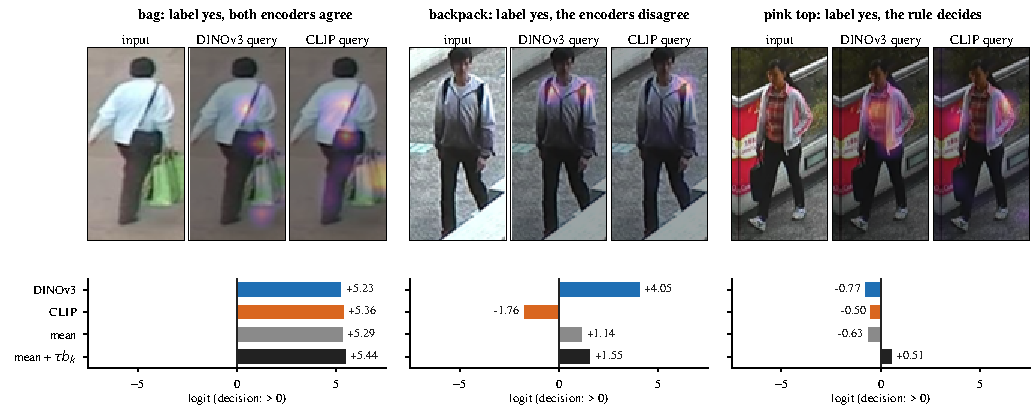
\includegraphics[width=\linewidth]{method_cases.pdf}
\caption{The method on three PETA images, for an encoder pair that never saw PETA. Top: input and the attention of each encoder's query for the named attribute. Bottom: the attribute logit of each encoder, their mean and the mean after the decision rule.}
\label{fig:method}
\end{figure*}

\subsection{Ensembling by logit averaging}
\label{sec:ensemble}

The two encoders produce one logit per attribute. We average the logits with equal weights, $\bar z_k=\tfrac12(z_k^{\text{DINO}}+z_k^{\text{CLIP}})$. Averaging logits rather than probabilities lets a confident member outvote an uncertain one, as in the backpack example of \cref{fig:method}, where DINOv3 is confidently right and CLIP is wrong with less confidence. Equal weights are a deliberate choice. The best weight depends on the target domain, which is unknown, and \cref{sec:design} shows that equal weights sit at the optimum of both held-out domains we can measure.

\subsection{One-coefficient decision rule}
\label{sec:rule}

The averaged logit still has to be turned into a yes or no at a threshold of 0.5. Per-attribute offsets fitted on the source validation data are the common fix, but they absorb the labelling conventions of the source datasets and are noisy, because each of the 40 offsets is estimated from few positives. A rule for an unseen domain should instead have few parameters and a target that does not depend on the label distribution of that domain.

The mA half of the metric provides such a target. Balanced accuracy weighs positives and negatives equally, so its Bayes-optimal decision is the one made under a balanced prior, whatever the true target prior is. If the model is calibrated under the training prior $\pi_k$, moving to a balanced prior adds $\log\frac{1-\pi_k}{\pi_k}$ to the logit~\cite{saerens,logitadj}. The DeepMAR weights have already moved the optimum of the training loss by $\log(w_k^{+}/w_k^{-})=1-2\pi_k$ in the same direction. The remaining correction is therefore
\begin{equation}
b_k=\log\frac{1-\pi_k}{\pi_k}-(1-2\pi_k),\qquad z_k \leftarrow \bar z_k+\tau\,b_k .
\label{eq:rule}
\end{equation}
Instance F1, the other half of the metric, prefers fewer positives for rare attributes. A shared coefficient $\tau\in[0,1]$ trades the two halves off. It interpolates between the decision of the weighted loss ($\tau=0$) and the mA-optimal decision ($\tau=1$). For a rare attribute such as a pink top ($\pi_k\approx0.02$), $b_k$ is large and positive, which is why the rule turns the correct but negative mean logit of the third example in \cref{fig:method} into a positive decision. For a frequent attribute such as trousers ($\pi_k\approx0.9$), $b_k$ is negative. We use $\tau=0.42$, a value set in earlier experiments with single models on the PETA-held-out protocol, and the priors $\pi_k$ of all training and validation labels. The derivation ignores label smoothing and assumes calibration under $\pi_k$, so it motivates the form of the rule rather than fixing $\tau$.

%=====================================================================
\section{Experimental Protocol}
\label{sec:protocol}

\paragraph{Held-out domains.} In-domain validation scores say little about an unseen domain. We therefore train on the training splits of two datasets and evaluate on the validation split of the third. PETA is the main held-out domain, because its ten pooled sources make it the most varied of the three. Market1501 serves as a second held-out domain for the key comparisons. For the PETA-held-out models we also report an in-domain score on the Market1501 and PA100k validation images, which the models did not see during training. All held-out numbers apply the decision rule with the priors of the training folds. Mean AUC over attributes measures ranking independently of any threshold. Protocol models are trained for three epochs on two datasets, and the submitted models for three epochs on the training and validation splits of all three.

\paragraph{Noise.} Four CLIP ViT-L/14 runs with the same recipe differ only in seed, machine or activation implementation. On PETA held out they score between 81.13 and 81.58, and paired with the same DINOv3 model between 82.17 and 82.42. Differences between single protocol runs below about 0.3\pts{} are therefore not reliable, and we require larger margins before changing the system.

%=====================================================================
\section{Experiments}
\label{sec:experiments}

\subsection{Which encoders to pair}
\label{sec:pairing}

We fine-tuned ten foundation encoders with the recipe of \cref{sec:encoders} and paired each with DINOv3 ViT-H+ (\cref{tab:encoders}). CLIP ViT-L/14 is the best partner on both the held-out and the in-domain readout, and the closely related MetaCLIP ViT-L/14~\cite{metaclip} is second. Ranking quality alone does not make a good partner. Both SigLIP2 encoders~\cite{siglip2} rank PETA attributes about as well as CLIP, with a similar AUC, but form two of the four weakest pairs. Across the nine partners, the partner's own Avg predicts the pair's Avg with a Spearman correlation of 0.92, while its AUC reaches only 0.42. Compared with CLIP, the SigLIP2 encoders produce more false positives on rare attributes such as glasses, old age and baldness, and averaging with DINOv3 does not remove them. The partner should therefore be chosen by its thresholded accuracy on a held-out domain, and among the encoders we tried, the CLIP family is the clear choice.

\begin{table}[t]
\centering\small
\setlength{\tabcolsep}{2.6pt}
\resizebox{\columnwidth}{!}{%
\begin{tabular}{@{}llccccc@{}}
\toprule
& & \multicolumn{3}{c}{single encoder} & \multicolumn{2}{c}{with DINOv3-H+} \\
\cmidrule(lr){3-5}\cmidrule(l){6-7}
Encoder & Input & PETA & AUC & in-dom. & PETA & in-dom. \\
\midrule
DINOv3 ViT-H+/16~\cite{dinov3} & 224$\times$112 & 81.42 & 92.23 & 88.66 & -- & -- \\
\midrule
CLIP ViT-L/14~\cite{clip} & 224$\times$112 & 81.54 & 91.87 & 88.38 & 82.33 & 89.14 \\
MetaCLIP ViT-L/14~\cite{metaclip} & 224$\times$112 & 81.35 & 92.04 & 88.51 & 82.14 & 89.19 \\
EVA02-CLIP ViT-L/14~\cite{evaclip} & 224$\times$112 & 80.58 & 90.97 & 87.94 & 82.03 & 89.02 \\
AIMv2 ViT-L/14~\cite{aimv2} & 224$\times$112 & 80.23 & 91.40 & 87.82 & 81.90 & 88.96 \\
PE-Core ViT-L/14~\cite{pe} & 224$\times$112 & 80.71 & 91.23 & 88.06 & 81.88 & 89.02 \\
MetaCLIP2 ViT-H/14~\cite{metaclip2} & 168$\times$84 & 80.42 & 91.63 & 87.29 & 81.87 & 88.84 \\
SigLIP2 So400m/14~\cite{siglip2} & 224$\times$112 & 80.12 & 91.67 & 87.60 & 81.86 & 88.94 \\
SigLIP2 ViT-L/16~\cite{siglip2} & 256$\times$128 & 80.12 & 91.76 & 87.81 & 81.68 & 89.01 \\
DFN-CLIP ViT-L/14~\cite{dfn} & 224$\times$112 & 79.37 & 90.87 & 86.95 & 81.63 & 88.78 \\
\bottomrule
\end{tabular}}
\caption{Encoders alone and paired with DINOv3 ViT-H+ by logit averaging. PETA is held out during training, in-domain is the Market1501 and PA100k validation data.}
\label{tab:encoders}
\end{table}

\subsection{How to combine the pair}
\label{sec:design}

\Cref{tab:design} tests three alternatives to the equal-weight pair. The first changes the member weights. On PETA held out the optimum is at equal weights, while on Market1501 held out it moves towards DINOv3, which alone is as good as any mixture there. Equal weights lose at most 0.11\pts{} to the best weight on either domain, whereas committing to a single encoder loses up to 0.91\pts{} on one of them. Without knowledge of the target domain, equal weights are the safe choice.

The second alternative adds a third member. None of the four candidates improves the pair, including MetaCLIP2 ViT-H/14, the largest encoder we tried. A third member mostly adds a model similar to one already present, and on a thresholded metric its own false positives count as much as its corrections.

The third alternative replaces the pair by one encoder of the same size. We distilled an ensemble of DINOv3 ViT-H+, CLIP ViT-L/14 and MetaCLIP2 ViT-H/14 into a DINOv3 ViT-H+ student with soft-target distillation~\cite{hinton} on mixed inputs for 15 epochs. The student is as accurate as the best single encoder of this study. Pairing it with CLIP, however, gains less than pairing the original DINOv3 model with CLIP, because the student has already absorbed CLIP's predictions and no longer disagrees with it. When the inference budget allows two encoders, an ensemble of independently fine-tuned members is the better use of it.

\begin{table}[t]
\centering\small
\setlength{\tabcolsep}{4pt}
\begin{tabular}{@{}lcc@{}}
\toprule
Variant & PETA & Market1501 \\
\midrule
DINOv3-H+ + CLIP-L, equal weights & 82.33 & 86.35 \\
\quad weight of DINOv3-H+ 0.4 & 82.30 & 86.23 \\
\quad weight of DINOv3-H+ 0.6 & 82.29 & 86.46 \\
\quad DINOv3-H+ alone & 81.42 & 86.46 \\
\quad CLIP-L alone & 81.54 & 85.60 \\
\midrule
+ MetaCLIP ViT-L/14 & 82.32 & -- \\
+ MetaCLIP2 ViT-H/14 & 82.27 & -- \\
+ AIMv2 ViT-L/14 & 82.16 & -- \\
+ SigLIP2 So400m/14 & 82.15 & -- \\
\midrule
distilled DINOv3-H+ student alone & 82.00 & -- \\
distilled student + CLIP-L & 82.21 & -- \\
\bottomrule
\end{tabular}
\caption{Alternatives to the equal-weight pair, with each domain held out during training.}
\label{tab:design}
\end{table}

\subsection{How far to adapt the encoders}
\label{sec:depth}

Our recipe freezes eight blocks and uses a steep layer decay. A natural question is whether the encoders, especially the 32-block DINOv3 ViT-H+, are under-trained by it. We compare it with a deeper recipe that freezes four blocks and uses $\gamma=0.9$ instead of eight blocks and $\gamma=0.75$, which gives the middle blocks of ViT-H+ about twenty times larger learning rates (\cref{tab:depth}). The deeper recipe raises the in-domain score of every encoder. On the held-out domains the picture is mixed. It helps DINOv3 and SigLIP2, leaves CLIP unchanged on Market1501 and costs it 0.44\pts{} on PETA. In the ensemble, the held-out gains shrink to 0.07--0.18\pts, within the noise of \cref{sec:protocol}, and \cref{sec:test} shows that they do not appear on the hidden test. Deeper adaptation thus fits the source domains better without a reliable benefit on unseen ones, so we keep the conservative recipe.

\begin{table}[t]
\centering\small
\setlength{\tabcolsep}{3.2pt}
\resizebox{\columnwidth}{!}{%
\begin{tabular}{@{}lccc@{}}
\toprule
Model & in-domain & PETA held out & Market1501 held out \\
\midrule
DINOv3 ViT-H+/16 & 88.66 $\rightarrow$ 89.17 & 81.42 $\rightarrow$ 82.01 & 86.46 $\rightarrow$ 86.64 \\
CLIP ViT-L/14 & 88.38 $\rightarrow$ 88.82 & 81.54 $\rightarrow$ 81.10 & 85.60 $\rightarrow$ 85.63 \\
SigLIP2 ViT-L/16 & 87.81 $\rightarrow$ 88.60 & 80.12 $\rightarrow$ 81.09 & -- \\
\midrule
Ensemble (deeper DINOv3) & 89.14 $\rightarrow$ 89.35 & 82.33 $\rightarrow$ 82.51 & 86.35 $\rightarrow$ 86.42 \\
\bottomrule
\end{tabular}}
\caption{Conservative recipe $\rightarrow$ deeper recipe, single encoders and the ensemble.}
\label{tab:depth}
\end{table}

\subsection{The decision rule}
\label{sec:rule_exp}

\Cref{fig:tau} plots Avg against $\tau$ on both held-out domains. On PETA the rule raises the ensemble by 1.24\pts{} over the plain threshold, and on Market1501 by 0.84\pts. The two single encoders gain by similar amounts, so the rule and the ensemble act on different parts of the error and their gains add up. All curves rise until $\tau$ reaches 0.5 to 0.65 and collapse soon after, when rare attributes are predicted far too often and instance F1 breaks down. The value $\tau=0.42$, chosen before these models existed, lies on the rising part on both domains, close to the best value and safely away from the collapse.

To measure what thresholds could still gain, we fit per-attribute offsets on the held-out labels themselves. This oracle cannot be used at test time, but its gain over the rule bounds what any threshold rule could recover. It is 1.85\pts{} on PETA and 1.70\pts{} on Market1501 for the ensemble. The remaining threshold error is thus larger than any gain from the choice of encoders in \cref{tab:encoders}. In earlier work on this protocol we traced most of it to clothing colors, whose labelling differs between datasets. PETA, for instance, marks two colors for 12\% of upper garments, whereas the other datasets almost never do. Source data cannot recover this part of the error, which is the main limitation of every system that, like ours, may not use target images.

\begin{figure}[t]
\centering
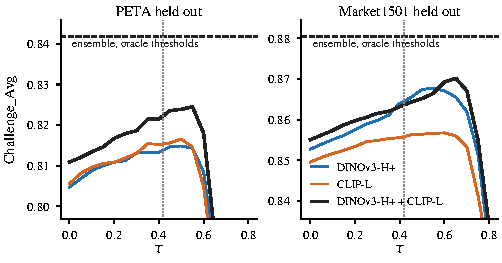
\includegraphics[width=\linewidth]{tau_rule.pdf}
\caption{Challenge\_Avg as a function of the decision-rule coefficient $\tau$ on two held-out domains. The dotted line marks the submitted value and the dashed line the ensemble with thresholds fitted on the held-out labels.}
\label{fig:tau}
\end{figure}

\subsection{Hidden-test results}
\label{sec:test}

\Cref{tab:test} lists our main submissions with the PETA-held-out score of the same recipe. The protocol ranks the first three submissions in the order of their test scores. Moving from a single distilled DINOv3 ViT-L to an ensemble of four models gains 0.63\pts{} on the test set. The protocol score of v20 uses the ten-epoch student of v13 in place of its longer-trained student. Replacing that ensemble by the DINOv3 ViT-H+ and CLIP ViT-L pair, which is both smaller and better on the protocol, gains a further 0.22\pts. The fourth submission is the deeper recipe of \cref{sec:depth}. Its protocol gain of 0.18\pts{} is inside the noise band, and on the test it loses 0.10\pts. This is the outcome the noise estimate predicts for such a margin. The submitted system v21 reaches an mA of 80.61 and an instance F1 of 79.33, with precision 75.61 and recall 84.90.

\begin{table}[t]
\centering\small
\setlength{\tabcolsep}{3pt}
\resizebox{\columnwidth}{!}{%
\begin{tabular}{@{}llcc@{}}
\toprule
& Members & PETA held out & Hidden test \\
\midrule
v13 & distilled DINOv3 ViT-L/16 student & 81.18 & 79.12 \\
v20 & student + DINOv3 ViT-L + CLIP-L + MetaCLIP2-H & 82.03 & 79.75 \\
v21 & DINOv3 ViT-H+ + CLIP ViT-L (this paper) & 82.33 & 79.97 \\
v22 & v21 with deeper DINOv3 fine-tuning & 82.51 & 79.87 \\
\bottomrule
\end{tabular}}
\caption{Submissions to UPAR 2027 Track~1 and the protocol scores of their recipes.}
\label{tab:test}
\end{table}

%=====================================================================
\section{Conclusion}
\label{sec:conclusion}

On unseen cameras, attribute recognition fails through ranking and through thresholds, and the two call for different components. For ranking, two conservatively fine-tuned encoders from different pretraining families, chosen by thresholded held-out accuracy and averaged with equal weights, outperform larger ensembles, distilled single models and more deeply fine-tuned variants. For thresholds, one coefficient applied to a prior-dependent term recovers more than a point of the challenge score, while a larger threshold error remains that source data cannot remove.

\paragraph{Limitations.} Most comparisons rest on one held-out dataset and one training run per configuration, and the noise estimate comes from a single encoder. \Cref{fig:method} illustrates the method with smaller members than the submitted ones. The decision rule assumes priors estimated from representative training data, and its coefficient was set on held-out data from the training datasets.

\paragraph{Broader impact.} Attribute recognition on surveillance video, including age and gender, can support tracking of individuals. We report technical findings only and do not release models trained on surveillance data.

{\small
\bibliographystyle{ieeenat_fullname}
\bibliography{refs}
}

%=====================================================================
\clearpage
\appendix
\section{Training configuration}
\label{app:config}

Both encoders use the same recipe. Optimizer AdamW with learning rate $5\cdot10^{-5}$ at the last block, layer decay $\gamma=0.75$, head learning rate ten times larger, weight decay 0.05, batch size 64, cosine schedule with half an epoch of warm-up, stochastic depth 0.1, three epochs, bf16 mixed precision and an exponential moving average of the weights with decay 0.9995, which is the model used at test time. The query head has one layer, eight attention heads, an MLP ratio of two and dropout 0.1. Augmentation consists of random down-scaling to simulate low-resolution crops, horizontal flip, edge padding of ten pixels followed by a random crop, brightness, contrast and saturation jitter without hue change, Gaussian blur and random erasing. Priors $\pi_k$ are clipped to $[10^{-3},1-10^{-3}]$. Cells that a dataset does not annotate are masked in the loss. The two submitted members are trained on the training and validation splits of all three datasets. At test time both read the same crop resized to $224\times112$, and the pair processes the 29{,}248 test images in about four minutes on one NVIDIA A10 GPU.

\end{document}
